\section{Prodigal Patterns}{\label{sec:prodigalpatterns}}
\begin{topics}
\verb!turtleSim! (turtle simulator) and its features \verb!forward, right, left, penUp, penDown!\\
\verb!repeat! statement, variables and their data types (\verb!int, char!), typecasting.
\end{topics}
\subsection{Star Spiral}{\label{pp:starspiral}}
\textbf{Problem Statement:}\\
Draw the following Star Spiral.
\begin{figure}[H]
	\centering
	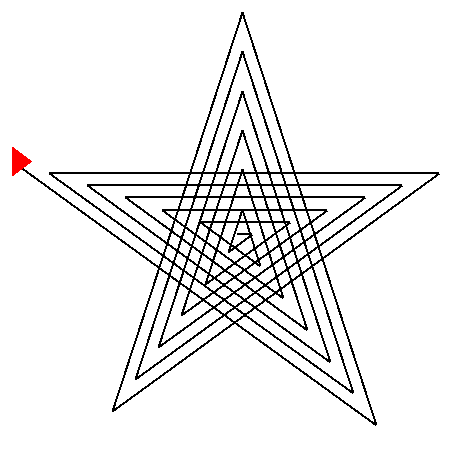
\includegraphics[width = 0.7\linewidth]{Star Spiral.png}
	\caption{A Star Spiral of 30 sides}
\end{figure}
\subsection{Peace}{\label{pp:peace}}
\textbf{Problem Statement:}\\
Draw the outline of the Proportionl Peace Sign according to measurements as shown in \ref{fig:peacemeasurements}.
\begin{figure}[H]
\centering
	\begin{subfigure}{\linewidth}
	\centering
	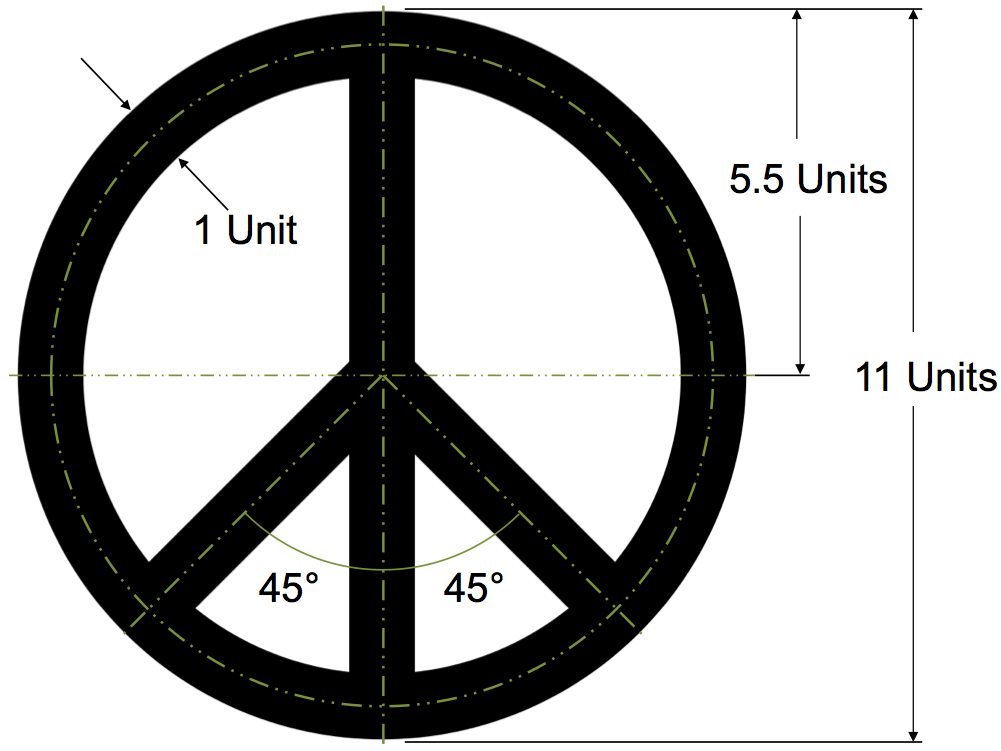
\includegraphics[width = 0.4\linewidth]{Peace Measurements.png}
	\caption{Measurements by Jerry S. Sadin, based on \href{https://bit.ly/peace-sign-measurements}{Peace Sign} by Schuminweb}
	\label{fig:peacemeasurements}
\end{subfigure}
\begin{subfigure}{\linewidth}
	\centering
	
\includegraphics[width = 0.65\linewidth]{Peace.png}
	\caption{Output generated using Simplecpp}
	\label{fig:peace}
\end{subfigure}
\caption{Peace Sign}
\end{figure}
The output image will look like \ref{fig:peace}.
\begin{funvideo}
\href{https://youtu.be/GO5FwsblpT8}{Carl Sagan's Pale Blue Dot -- carlsagandotcom}\\
\href{https://youtu.be/lshWT0iyxds}{Cosmos: Possible Worlds (Carl Sagan's Monologue) -- Evil Dead}
\end{funvideo}
\subsection{Butterfly}{\label{pp:butterfly}}
\textbf{Problem Statement:}\\
Print the Butterfly pattern for a general $n$. See Starter code (below) for more details.
\begin{testcases}
	{$t$ \hfill(number of test cases, an integer)\\
	$n_1\ n_2\ \ldots\ n_t$ \hfill($t$ space seperated integers for each testcase)}
	{Butterfly pattern \hfill(each test case on a newline)}
	{$1 \leq n_i \leq 10$}
	{5\\1 2 3 4 5}
	% {*\space\space\space*\newline*\space*\space*}
	{\vspace{-2em}
	\begin{figure}[H]
	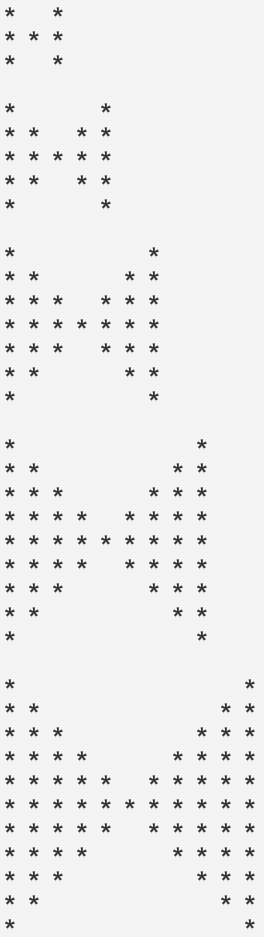
\includegraphics[scale=0.73]{Butterfly.png}
	\end{figure}
	% \begin{table}[H]
	% \begin{tabular}{p{0.001pt}p{0.001pt}p{0.001pt}p{0.001pt}p{0.001pt}}
	% * &  &   &  & * \\
	% * &  & * &  & * \\
	% * &  &   &  & *
	% \end{tabular}
	% \end{table}
	% \begin{table}[H]
	% \begin{tabular}{lllll}
	% * &  &   &  & * \\
	% * &  & * &  & * \\
	% * &  &   &  & *
	% \end{tabular}
	% \end{table}
	}
	{https://github.com/paramrathour/CS-101/tree/main/Starter Codes/Butterfly.cpp}
\end{testcases}
\begin{funvideo}
\href{https://youtu.be/fDek6cYijxI}{Chaos: The Science of the Butterfly Effect -- Veritasium}
\end{funvideo}
\subsection{Alphabetical Floyd's Triangle}{\label{pp:alphabeticalfloydstriangle}}
The alphabets are filled in alphabetical order (`A' to `Z') and a newline is started after printing $n$ alphabets on the $n$\textsuperscript{th} line. After `Z', the alphabets ``wrap around'' to `A'.

\textbf{Problem Statement:}\\
Print the left-aligned Alphabetical Floyd's Triangle for all given $n$. See Starter code (below) for more details.
\begin{testcases}
	{$t$ \hfill(number of test cases, an integer)\\$n_1\ n_2\ \ldots\ n_t$ \hfill($t$ space seperated integers for each testcase)}
	{Alphabetical Floyd's Triangle \hfill(left-aligned, each test case on a newline)}
	{$1 \leq n_i \leq 20$}
	{5\\1 2 3 5 17}
	{A\\\\A\\B C\\\\A\\B C\\D E F\\\\A\\B C\\D E F\\G H I J\\K L M N O\\\\A\\B C\\D E F\\G H I J\\K L M N O\\P Q R S T U\\V W X Y Z A B\\C D E F G H I J\\K L M N O P Q R S\\T U V W X Y Z A B C\\D E F G H I J K L M N\\O P Q R S T U V W X Y Z\\A B C D E F G H I J K L M\\N O P Q R S T U V W X Y Z A\\B C D E F G H I J K L M N O P\\Q R S T U V W X Y Z A B C D E F\\G H I J K L M N O P Q R S T U V W}
	{https://github.com/paramrathour/CS-101/tree/main/Starter Codes/Alphabetical Floyd's Triangle.cpp}
\end{testcases}
\subsection{Bernoulli's Triangle}{\label{pp:bernoullistriangle}}
You might have heard about \href{https://youtu.be/0iMtlus-afo}{Pascal's Triangle}. 
The $k$\textsuperscript{th} element of row $n$ of Bernoulli's Triangle is obtained by as shown in \ref{fig:bernoullistriangle} summing all elements of the row $n$ (row $0$ is the first row) until the $k$\textsuperscript{th} element (partial sums).
\begin{figure}[H]
	\centering
	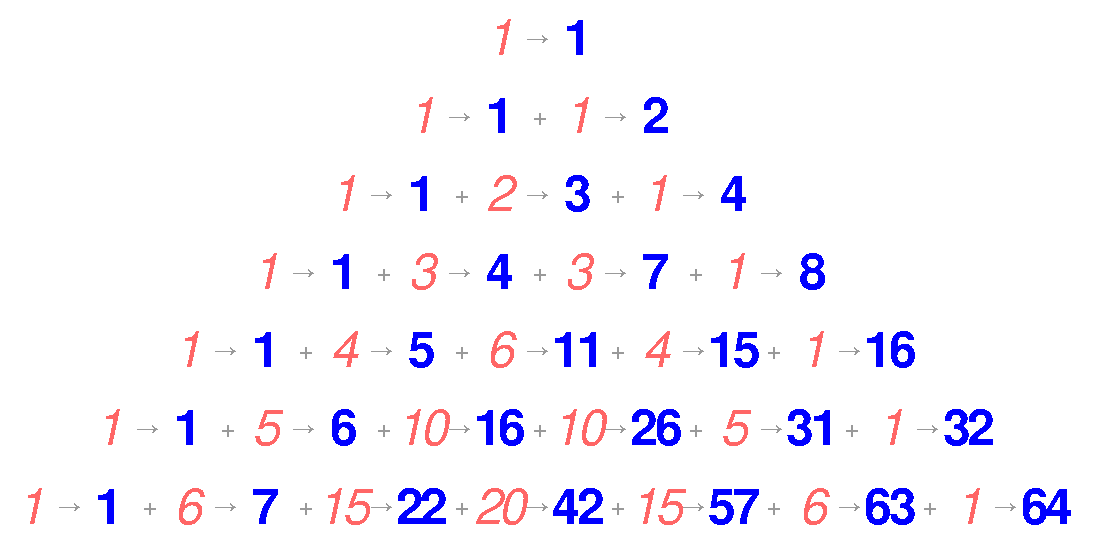
\includegraphics[width = 0.4\linewidth]{Bernoulli's Triangle.pdf}
	\caption{Bernoulli's triangle (\textbf{\textcolor{blue}{blue bold}} text) from Pascal's triangle (\textit{\textcolor{pink}{pink italics}}) (Drawn by CMG Lee, \href{https://bit.ly/bernoullis-triangle}{Image Source})}
	\label{fig:bernoullistriangle}
\end{figure}
% Formally given as below
% \begin{equation}
% B_{n,k} =  \sum _{p=0}^{k}{n \choose p}
% \end{equation}
\vspace{-1.5em}
\textbf{Problem Statement:}\\
Print the left-aligned Bernoulli's Triangle for all given $n$. See Starter code (below) for more details.
\begin{testcases}
	{$t$ \hfill(number of test cases, an integer)\\$n_1\ n_2\ \ldots\ n_t$ \hfill($t$ space seperated integers for each testcase)}
	{Bernoulli's Triangle \hfill(left-aligned, each test case on a newline)}
	{$0 \leq n_i \leq 20$}
	{4\\0 1 2 10}
	{1\\\\1\\1 2\\\\1\\1 2\\1 3 4\\\\1\\1 2\\1 3 4\\1 4 7 8\\1 5 11 15 16\\1 6 16 26 31 32\\1 7 22 42 57 63 64\\1 8 29 64 99 120 127 128\\1 9 37 93 163 219 247 255 256\\1 10 46 130 256 382 466 502 511 512\\1 11 56 176 386 638 848 968 1013 1023 1024}
	{https://github.com/paramrathour/CS-101/tree/main/Starter Codes/Bernoulli's Triangle.cpp}
\end{testcases}
\begin{funvideo}
\href{https://youtu.be/0iMtlus-afo}{Pascal's Triangle -- Numberphile}
\end{funvideo}